\documentclass[11pt]{article}

% Template-agnostic preamble.
\usepackage[margin=1in]{geometry}
\usepackage[utf8]{inputenc}
\usepackage[T1]{fontenc}
\usepackage{hyperref}
\hypersetup{colorlinks=true, linkcolor=blue, citecolor=blue, urlcolor=blue,
  pdftitle={The Lever Generalizes -- and It Brakes},
  pdfauthor={Anonymous}}
\emergencystretch=3em
\sloppy
\hyphenpenalty=2000
\exhyphenpenalty=0
\hbadness=10000
\usepackage{booktabs}
\usepackage{amsfonts}
\usepackage{amsmath}
\usepackage{amssymb}
\usepackage{xcolor}
\usepackage{array}
\usepackage{graphicx}

\title{The Lever Generalizes --- and It Brakes: \\
A Late, Bidirectional Action-Commitment Lever Across Agent Decisions and Architectures \\[2pt]
\large Toward mechanistic circuit-breakers for irreversible agent actions}

\author{Anonymous Submission \\ BlackboxNLP 2026 (under double-blind review)}
\date{June 2026}

\begin{document}
\maketitle

\begin{abstract}
A prior result (\emph{The Lever Is Late}) showed that, for a long-horizon coding agent, control of the
\texttt{finish} decision lives not at the mid-layer ``task is done'' verdict but in a late, task-matched
action-commitment block $\sim$30 layers downstream. That left two questions open: is the late lever
\emph{specific to termination}, and can it \emph{brake} an action, not just elicit one? We answer both on
Qwen3.6-27B over 99 SWE-bench Pro trajectories, using a second, distinct decision available in the same data
--- commit a file edit (\texttt{str\_replace\_editor}) versus continue reversible exploration (\texttt{bash})
--- with $n{=}60$ deterministic decision points per condition, prefill-only patching, and generation-confirmed
outcomes. \textbf{(1) Generalization (elicit).} At an explore decision, injecting a task-matched
\emph{edit}-donor into the late block makes the agent emit a real \texttt{edit} call: $0.23 \to 0.77$ at L59
(position control $0.08$, cross-task control $0.48$). \textbf{(2) The brake (suppress).} At a commit decision,
injecting an \emph{explore}-donor collapses the real edit rate $0.48 \to 0.02$ (96\% suppression) at L55, with
a same-class control intact ($0.55$) and the opposite-direction donor boosting to $0.92$. \textbf{(3) The
mechanism is monotonic and bidirectional.} Exact paired McNemar on all $14$ per-point conditions yields seven
contrasts that survive Holm--Bonferroni ($m{=}7$, worst $p{=}7.6\mathrm{e}{-}5$); the discordance structure is
the headline: elicit has $c{=}0$ (the edit-donor only \emph{turns commits on}, never silences) and the brake
has $b{=}0$ (the explore-donor only \emph{turns them off}, never lights). The late lever moves exactly in the
donor's direction with $\sim$zero off-direction noise. \textbf{(4) Cross-architecture.} The late-commitment
\emph{geometry} and a donor-specific late \emph{writability} replicate in a different model family
(Mistral-7B-Instruct-v0.3): the tool-commit decision is flat/negative through the first half and explodes in
the late block, and a task-matched edit-donor raises $P(\text{edit})$ where a same-norm random vector destroys
it. We frame the bidirectional late lever as the mechanism for a \emph{mechanistic circuit-breaker}: a single
late-layer intervention that blocks an action at its commit point. We demonstrate it on a state-mutating but
\emph{undoable} edit; intervening on a genuinely irreversible action (e.g.\ \texttt{send\_transaction}) is the
named next step. Tool, pre-registration, per-point data, and an adversarial pre-publication evaluation are
released.
\end{abstract}

\section{Background and contribution}\label{sec:bg}
Recent work~\cite{toolentropy,rightlocus,verdict,leverislate} established, across five studies on Qwen3.6-27B (a reasoning-tuned 27B model), a
detection--control asymmetry for long-horizon agent failure: internal states that \emph{predict} a behavior
routinely fail to \emph{control} it. A recent result~\cite{leverislate} located control of the
\texttt{finish} decision in a late action-commitment block (L51--L63), $\sim$30 layers downstream of the
mid-layer verdict, and only when steered with a \emph{task-matched} donor. We build on a model-agnostic steering tool implementing three primitives --- \textsc{locate} (logit-lens
per layer), \textsc{sweep\_patch} (donor injection per layer), and \textsc{steer\_generate} (prefill-only patch
of the decision position, then free decoding). This sits in the activation-steering / representation-engineering line~\cite{actadd,repe}, applied to a long-horizon agent's \emph{action channel} across turns rather than a single-turn attribute.

This paper pre-registers and answers two questions that the single \texttt{finish} result could not
(both pre-registrations are in the supplementary material). First, is the late lever a property of
the \emph{action-commitment channel} or an idiosyncrasy of termination? Second, can the lever \emph{suppress} an
action at its commit point --- the mechanism a safety \emph{circuit-breaker} would need? Our contributions:
\begin{enumerate}\itemsep1pt
  \item The late lever \textbf{generalizes} from \texttt{finish} to a second committal action (commit an edit),
    by the same locate--patch--steer method, generation-confirmed (\S\ref{sec:elicit}).
  \item The same lever \textbf{brakes}: a late explore-donor patch suppresses a real commit by 96\%
    (\S\ref{sec:brake}).
  \item The effect is \textbf{monotonic and bidirectional} --- elicit $c{=}0$, brake $b{=}0$ --- with all seven
    pre-registered contrasts surviving Holm--Bonferroni on exact paired McNemar (\S\ref{sec:stats}).
  \item The commitment \textbf{geometry and donor-specific writability replicate cross-family} on Mistral-7B
    (\S\ref{sec:xmodel}).
  \item We frame this as a \textbf{mechanistic circuit-breaker} and state honestly what is shown (a
    semi-irreversible proxy) and what is not (a genuinely irreversible action) (\S\ref{sec:disc}).
\end{enumerate}

\section{Setup}\label{sec:setup}
\textbf{Data and decision points.} We reuse the public bundle of 99 SWE-bench Pro~\cite{swebench} trajectories from
Qwen3.6-27B (success 40, locked 39, wandering 20). The agent's action space is three tools: \texttt{bash}
(3250 calls; reversible exploration), \texttt{str\_replace\_editor} (1101 calls; commits a file edit;
semi-irreversible), and \texttt{finish} (40). A \emph{commit decision point} is any turn poised between
committing an edit and continuing exploration; we reconstruct each faithfully at the tool-choice position,
deterministically (sorted traces, $\le 3$/trajectory), giving $n{=}60$ edit-decision and $n{=}60$
bash-decision points. \textbf{Patching.} All interventions use a prefill-only patching protocol: the late-position residual is replaced once at the decision token, then the model decodes greedily;
patching every step degenerates into repetition and is not used. \textbf{Fidelity gate.} Before any causal
number, $P(\text{edit})$ at reconstructed edit points ($0.474$) exceeds that at bash points ($0.299$), confirming
the states reproduce the real commit propensity (decision turns 5.2 vs 4.5 --- close, weakening a positional
confound; the position-matched control below addresses it directly).

\section{The late lever generalizes: eliciting a second action}\label{sec:elicit}
At a \texttt{bash} (explore) decision point we inject a task-matched \emph{edit}-donor late-block residual and
ask whether the agent emits a real \texttt{str\_replace\_editor} call (Table~\ref{tab:h1}). The baseline
emission rate is $0.23$; the task-matched edit-donor raises it to $0.77$ at L59. The two controls isolate the
effect: a \emph{position} control (an explore-donor at the same points) stays at $0.08$ --- below baseline,
ruling out ``any late patch elicits an edit'' --- and a \emph{cross-task} edit-donor reaches $0.48$, well above
baseline but below the task-matched donor. As in \emph{The Lever Is Late}, task-matching adds a real increment;
unlike \texttt{finish}, the \texttt{edit} decision also carries a substantial \emph{generic} component
(cross-task $\gg$ baseline), so task-specificity is \emph{graded per action}, not absolute.

\begin{table}[h]\centering\small
\begin{tabular}{lcc}
\toprule
condition (at bash decision points, $n{=}60$) & emission rate & exact McNemar vs.\ baseline \\
\midrule
no patch (baseline) & 0.23 & --- \\
task-matched edit-donor @L59 & \textbf{0.77} & $4.7\mathrm{e}{-}10$ ($b{=}32,c{=}0$) \\
task-matched edit-donor @L55 & 0.62 & $2.4\mathrm{e}{-}7$ ($b{=}23,c{=}0$) \\
position control (explore-donor) @L59 & 0.08 & --- (vs.\ donor: $9.1\mathrm{e}{-}13$) \\
cross-task edit-donor @L59 & 0.48 & --- (vs.\ donor: $7.6\mathrm{e}{-}5$) \\
\bottomrule
\end{tabular}
\caption{Elicit. A task-matched late edit-donor makes a stuck-in-exploration agent emit a real edit call.}
\label{tab:h1}
\end{table}

\section{The same lever brakes: suppressing a commit}\label{sec:brake}
At an \texttt{edit} (commit) decision point we inject an \emph{explore}-donor and measure whether the real edit
emission is suppressed (Table~\ref{tab:h2}). The baseline edit rate is $0.48$; the explore-donor at L55
collapses it to $0.02$ --- a 96\% suppression. The controls are clean: a same-class (edit-donor) patch at L55
does \emph{not} suppress (0.55), and the opposite intervention --- a task-matched edit-donor at L59 --- pushes
the rate \emph{up} to 0.92. Thus L55 is the brake point and L59 the power point ($0.03 \leftrightarrow 0.92$; Figure~\ref{fig:bidir}). A
generation-confirmed, single late-layer patch blocks a real commit.

\begin{table}[h]\centering\small
\begin{tabular}{lcc}
\toprule
condition (at edit decision points, $n{=}60$; baseline edit rate 0.48) & edit rate & exact McNemar \\
\midrule
explore-donor (brake) @L55 & \textbf{0.02} & $7.5\mathrm{e}{-}9$ ($b{=}0,c{=}28$) \\
explore-donor (brake) @L59 & 0.03 & $1.5\mathrm{e}{-}8$ ($b{=}0,c{=}27$) \\
same-class control (edit-donor) @L55 & 0.55 & --- \\
opposite (edit-donor) @L59 & 0.92 & --- \\
\bottomrule
\end{tabular}
\caption{Brake. A late explore-donor patch suppresses a real commit; same-class control intact.}
\label{tab:h2}
\end{table}

\begin{figure}[h]\centering
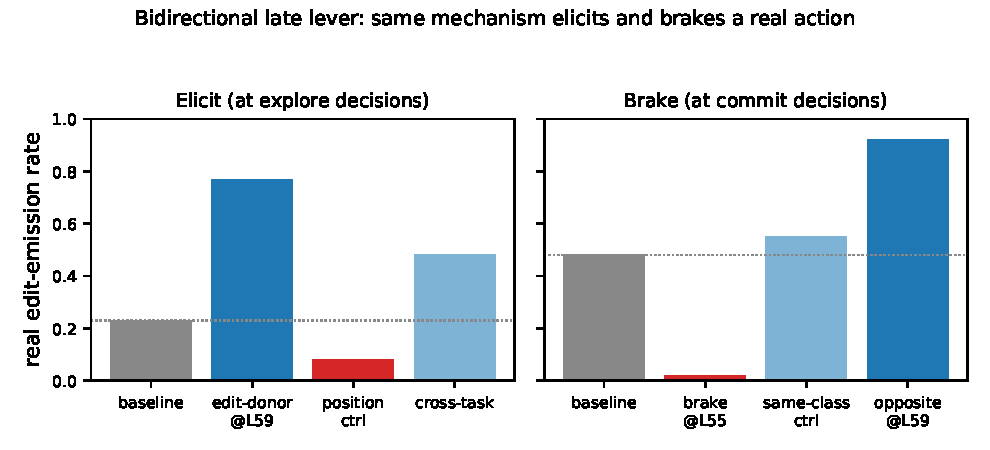
\includegraphics[width=0.74\textwidth]{figures/fig3_bidirectional.pdf}
\caption{The same task-matched late lever elicits a real edit at an explore decision (left) and brakes a real
edit at a commit decision (right), each against position / same-class and cross-task / opposite controls.}
\label{fig:bidir}
\end{figure}

\section{The mechanism is monotonic and bidirectional}\label{sec:stats}
We logged the per-point binary outcome for all 14 conditions and computed exact two-sided paired McNemar~\cite{mcnemar}
tests. All seven pre-registered contrasts survive Holm--Bonferroni~\cite{holm} ($m{=}7$; worst, task-specificity,
$p{=}7.6\mathrm{e}{-}5$). The discordance structure is the result: every elicit contrast has $\mathbf{c{=}0}$
(the edit-donor turns commits \emph{on}, $b{=}23$--$41$, and \emph{never} silences one that already fired),
and every brake contrast has $\mathbf{b{=}0}$ (the explore-donor turns commits \emph{off}, $c{=}27$--$32$, and
\emph{never} lights one). The late lever therefore moves the decision \emph{exactly} in the donor's direction
with $\sim$zero off-direction noise --- a structural, not merely a rate-shift, claim. The one-token $\Delta
P(\text{edit})$ profile corroborates: monotonic from L23 ($-0.003$) to L63 ($+0.685$), with mid layers (L23,
L31) inert and the explore-donor control going \emph{negative} late ($-0.28$) --- the one-token signature of the
brake (Figure~\ref{fig:qwen}).

\begin{figure}[h]\centering
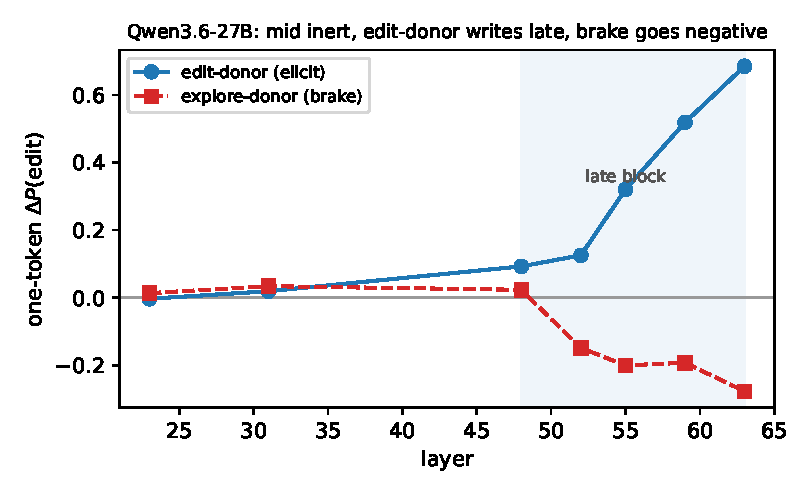
\includegraphics[width=0.62\textwidth]{figures/fig1_qwen_dprofile.pdf}
\caption{One-token $\Delta P(\text{edit})$ by layer (Qwen3.6-27B). The edit-donor (elicit) is inert mid-stream
and rises monotonically to L63; the explore-donor (brake) goes \emph{negative} in the same late block. The
lever is late, and bidirectional.}
\label{fig:qwen}
\end{figure}

\section{Cross-architecture replication}\label{sec:xmodel}
To test whether the late-commitment geometry is architectural rather than Qwen-specific, we ran a lite
locate-plus-one-token test on \texttt{Mistral-7B-Instruct-v0.3} (a distinct model family) over 30 SWE-bench Pro
tasks, with context-defined edit- vs.\ explore-decision points. \textbf{Geometry (robust over three runs):}
the logit-lens edit gap is flat/negative through the first half (L1--L15, $\sim-2$) and explodes in the late
block (L19 $+3.2$, L23 $+6.8$, L27 $+10.3$) --- the same mid-flat, late-explosion shape as Qwen.
\textbf{Writability:} injecting a task-matched edit-context donor into an explore decision raises
$P(\text{edit})$ donor-specifically (e.g.\ $+0.15$ at L27), whereas a same-norm \emph{shuffled} vector
\emph{lowers} it ($-0.61$ at L27); the donor-specific margin is $+0.6$--$0.76$ in the late block. The donor is
inert at L9/L11 and writes from L13 on. Two honest differences from the 27B result: the writable window begins
mid-depth ($\sim$L13, 40\%) rather than late-only, and this lite test omits generation confirmation. The
qualitative pattern --- a late-emerging, direction-specific, written-not-destroyed commitment representation
--- replicates across families (Figure~\ref{fig:xmodel}).

\begin{figure}[h]\centering
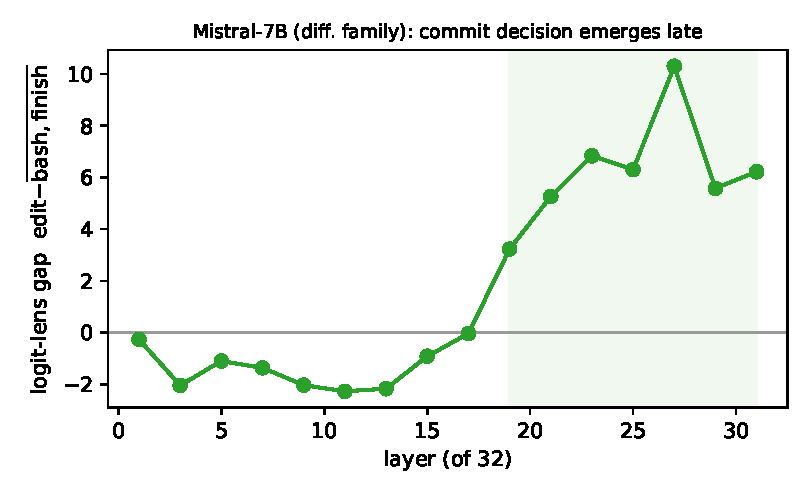
\includegraphics[width=0.62\textwidth]{figures/fig2_xmodel_locate.pdf}
\caption{Cross-family LOCATE (Mistral-7B-Instruct-v0.3). The logit-lens commit-vs-explore gap is flat/negative
through the first half and explodes in the late block (shaded) --- the same late-emergence geometry as
Qwen3.6-27B, in a different architecture.}
\label{fig:xmodel}
\end{figure}

\section{Discussion: a mechanistic circuit-breaker, and its honest scope}\label{sec:disc}
The bidirectional late lever is the mechanism a safety \emph{circuit-breaker} requires: a single intervention
at an action's commit point that can block it. We emphasize what is and is not shown.
\begin{itemize}\itemsep1pt
  \item \textbf{Generalization is an existence proof, not a universal law.} It holds for \texttt{finish} and
    one second action, on one model and one task family (plus a cross-family geometry/writability replication).
    More actions, models, and task families remain.
  \item \textbf{The proxy is semi-irreversible.} \texttt{str\_replace\_editor} mutates state but is undoable.
    The genuinely irreversible case (\texttt{send\_transaction}, \texttt{delete}) is untested and is the named
    next step; the circuit-breaker is demonstrated \emph{on a proxy}.
  \item \textbf{The brake redirect is uncontrolled.} Under the brake, \texttt{bash} is the dominant action
    (0.60), but we did not measure the no-brake bash baseline at edit points, so the redirect \emph{magnitude}
    is not established --- we report the brake-state composition, not ``routes to exploration''.
  \item \textbf{Emission is tool-token onset.} The elicit rate counts the tool-name prefix in a 16-token greedy
    continuation; some onsets are malformed, so $0.77$ is an upper bound on valid-call elicitation. The brake
    direction (suppression to $0.02$) is robust to this.
\end{itemize}
These caveats were produced by an adversarial pre-publication evaluation (in the supplementary material)
that recomputed every number from the released per-point data (determinism confirmed) and corrected two
earlier overclaims; we release it alongside the paper.

\paragraph{Relation to prior work.} This extends activation steering / patching from single-turn
representations to a long-horizon agent's action channel, and operationalizes the knowledge--action gap as a
\emph{layer} gap with a \emph{bidirectional} late lever --- consistent with recent work's detection$\neq$control
thesis and with mechanistic-corrigibility framings of pausing before irreversible actions.

\section{Conclusion}
The late action-commitment lever is not specific to termination and is not one-directional: a single
task-matched late patch both elicits and brakes a real agent action, monotonically and donor-specifically, with
a geometry that replicates across model families. This is the mechanism for a mechanistic circuit-breaker. The
next step is to demonstrate it on a genuinely irreversible action and at scale-matched second models.

\paragraph{Artifacts.} The model-agnostic steering tool, the two pre-registrations, the per-point data and deterministic decision-point state, the exact-statistics script, and the adversarial pre-publication evaluation are provided in the supplementary material and will be released publicly upon acceptance.

\begin{thebibliography}{99}
\bibitem{leverislate} Anonymous. The Lever Is Late: Causal Control of Long-Horizon Agent Termination Lives in a Task-Matched, Late Action-Commitment Block. 2026. (citation anonymized for review)
\bibitem{toolentropy} Anonymous. Tool-Entropy Collapse: A Cross-Architecture Signature of Agent Failure. 2026. (anonymized for review)
\bibitem{rightlocus} Anonymous. Causal Localization of Agent Non-Termination: The Right Locus Is Still Not a Rescue Lever. 2026. (anonymized for review)
\bibitem{modality} Anonymous. Modality Matters: A Transient Behavioral Interruption Rescues Agent Non-Termination Where Residual Steering Does Not. 2026. (anonymized for review)
\bibitem{verdict} Anonymous. The Verdict Is Not the Lever: An Interpretable Task-Completion Feature Predicts but Does Not Cause Long-Horizon Agent Termination. 2026. (anonymized for review)
\bibitem{actadd} A.~M.~Turner, L.~Thiergart, G.~Leech, D.~Udell, J.~J.~Vazquez, U.~Mini, M.~MacDiarmid. Activation Addition: Steering Language Models Without Optimization. arXiv:2308.10248, 2023.
\bibitem{repe} A.~Zou et al. Representation Engineering: A Top-Down Approach to AI Transparency. arXiv:2310.01405, 2023.
\bibitem{swebench} C.~E.~Jimenez, J.~Yang, A.~Wettig, S.~Yao, K.~Pei, O.~Press, K.~Narasimhan. SWE-bench: Can Language Models Resolve Real-World GitHub Issues? ICLR 2024. arXiv:2310.06770.
\bibitem{logitlens} nostalgebraist. Interpreting GPT: the Logit Lens. LessWrong, 2020.
\bibitem{mcnemar} Q.~McNemar. Note on the sampling error of the difference between correlated proportions or percentages. Psychometrika, 12(2):153--157, 1947.
\bibitem{holm} S.~Holm. A Simple Sequentially Rejective Multiple Test Procedure. Scandinavian Journal of Statistics, 6(2):65--70, 1979.
\end{thebibliography}

\end{document}
